%%%%%%%%%%%%%%%%%%%%%%%%%%%%%%%% PIPELINE %%%%%%%%%%%%%%%%%%%%%%%%%%%%%%%%

\lecture{Pipeline de Instruções}{pipeline}

\lecturetitle{\insertlecture}{\course}

\frame{\maketitle}

\def\thetitle{Introdução}

\section{\thetitle}

\frame{\author{}\title{\thetitle}\institute{}\date{}\titlepage}

\def\thescale{.25}
\begin{frame}{Vamos lavar a roupa suja}{\only<3>{Comparação}}
  \only<1,2>{ Execução das tarefas \alert{\underline{\only<1>{sem}\only<2>{com}} sobreposição}.}

  \begin{center}
    \includegraphics[scale=.35]<1>{img/pipeline-laundry_nopipe}
    \includegraphics[scale=.35]<2>{img/pipeline-laundry_pipe}
    \includegraphics[scale=\thescale]<3>{img/pipeline-laundry_nopipe}\\
    \includegraphics[scale=\thescale]<3>{img/pipeline-laundry_pipe}
  \end{center}  
\end{frame}

\section{Pipeline}

\frame{\LARGE \insertlecture}

\begin{frame}{Pipeline}
  \begin{flushright}
  \begin{quote}
    ``A vida já é curta e nós a encurtamos ainda mais desperdiçando o
    tempo.'' Victor Hugo
  \end{quote}
  \end{flushright}

  \begin{definition}
    Técnica de implementação da execução das instruções na qual múltiplas instruções são
    sobrepostas durante o ciclo do {\em clock}.
  \end{definition}

\end{frame}


\begin{frame}{Tempo total para cada instrução}

\footnotesize
Estágios de tarefas do processador MIPS:
\begin{enumerate}
\item {\bf IF} -- ``pegar'' ({\em fetch}) a instrução;
\item {\bf REGr} -- ler o registrador;
\item {\bf ULA} -- realizar a operação;
\item {\bf MEM} -- acessar os dados na memória;
\item {\bf REGw} -- gravar no registrador.
\end{enumerate}
\bigskip
\pause
  \begin{tabular}{|c|c|c|c|c|c|c|}\hline
    \bf Classe da instrução & \bf IF & \bf REGr & \bf ULA & \bf MEM &
    \bf REGw & \bf Total
    \\\hline\hline
    Load word ({\tt lw}) & 200 ps & 100 ps & 200 ps & 200 ps & 100 ps
    & 800 ps \\\hline
    Store word ({\tt sw}) & 200 ps & 100 ps & 200 ps & 200 ps & 
    & 700 ps \\\hline
    Formato-R ({\tt add},{\tt sub}) & 200 ps & 100 ps & 200 ps &  & 100 ps
    & 600 ps \\\hline
    Desvio ({\tt beq}) & 200 ps & 100 ps & 200 ps &  & 
    & 500 ps \\\hline
  \end{tabular}
  
\end{frame}

\begin{frame}{Ciclo único sem {\em pipeline}}
  \footnotesize
  
  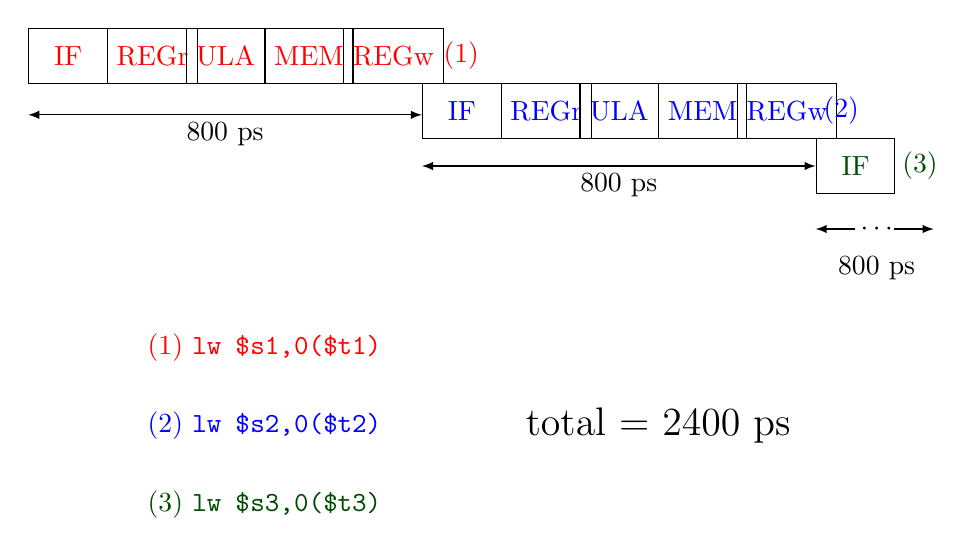
\begin{tikzpicture}
    \tikzset{inst/.style={rectangle,minimum height=.7cm,minimum width=1cm,anchor=west,draw}}

    \foreach \i/\l in {0/IF,1/REGr,2/ULA,3/MEM,4/REGw}{
      \node<1->[inst] at (\i,.7) {{\color{red}\l}};
      \node<2->[inst] at (5+\i,0) {{\color{blue}\l}};
    }
    
    \node<1-> at (5.5,.7) {{\color{red}(1)}};
    \draw<1->[<->,>=latex] (0,-.05) -- (5,-.05);
    \node<1-> at (2.5,-.3) {800 ps};

    \node<2-> at (10.325,0) {{\color{blue}(2)}};
    \draw<2->[<->,>=latex] (5,-.7) -- (10,-.7);
    \node<2-> at (7.5,-.95) {800 ps};
        
    \node<3-> at (11.325,-.7) {{\color{green!30!black}(3)}};
    \node<3->[inst] at (10,-.7) {{\color{green!30!black}IF}};
    \draw<3->[<-,>=latex] (10,-1.5) -- (10.5,-1.5);
    \node<3->[] at (10.775,-1.5) {$\cdots$};
    \draw<3->[->,>=latex] (11,-1.5) -- (11.5,-1.5);
    \node<3-> at (10.775,-2) {800 ps};
    
    % instrucoes
    \node<1-> (fi) at (3,-3) {{\color{red}(1) {\tt lw \$s1,0(\$t1)}}};
    \node<2-> (si) [below of=fi] {{\color{blue}(2) {\tt lw \$s2,0(\$t2)}}};
    \node<3-> [below of=si] {{\color{green!30!black}(3) {\tt lw \$s3,0(\$t3)}}};
    \node<3-> [right of=si, xshift=40mm] {\Large total = 2400 ps};

  \end{tikzpicture}
\end{frame}

\begin{frame}{Ciclo único com {\em pipeline}}
  \footnotesize
  REGw - escrita é feita na primeira metade do ciclo\\
  REGr -- leitura é feita na segunda metade do ciclo\\
\bigskip
  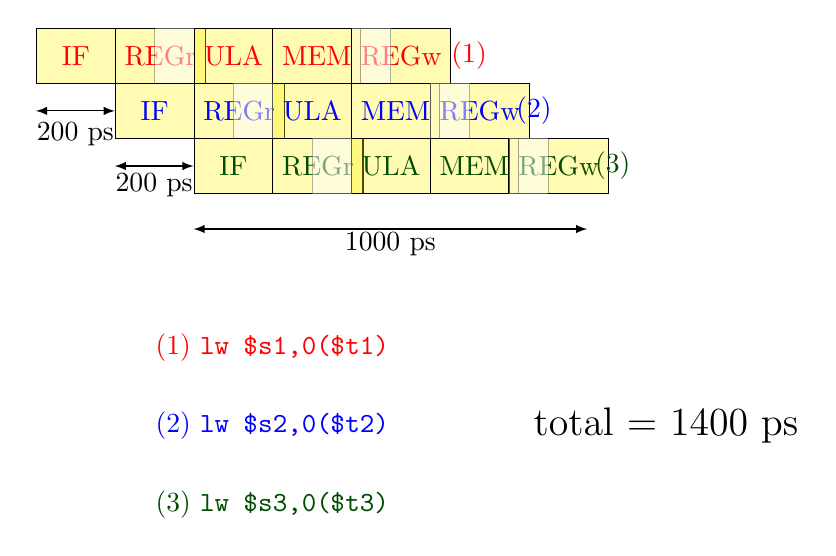
\begin{tikzpicture}
    \tikzset{inst/.style={rectangle,minimum height=.7cm,minimum
        width=1cm,anchor=west,fill=yellow,fill opacity=0.3,text opacity=1,draw},
    reg/.style={inst,minimum width=.5cm,fill=white,fill opacity=0.5,
     draw opacity=0.3}}

    \foreach \i/\l in {0/IF,1/REGr,2/ULA,3/MEM,4/REGw}{
      \node<1->[inst] at (\i,.7) {{\color{red}\l}};
      \node<2->[inst] at (1+\i,0) {{\color{blue}\l}};
      \node<3->[inst] at (2+\i,-.7) {{\color{green!30!black}\l}};
    }
    
    \node<1-> at (5.5,.7) {{\color{red}(1)}};
    \draw<1->[<->,>=latex] (0,0) -- (1,0);
    \node<1-> at (0.5,-.3) {200 ps};
    \node<1->[reg] at (1.5,.7) {};
    \node<1->[reg] at (4,.7) {};

    \node<2-> at (6.325,0) {{\color{blue}(2)}};
    \draw<2->[<->,>=latex] (1,-.7) -- (2,-.7);
    \node<2-> at (1.5,-.95) {200 ps};
    \node<2->[reg] at (2.5,0) {};
    \node<2->[reg] at (5,0) {};
    

    \node<3-> at (7.325,-.7) {{\color{green!30!black}(3)}};

    \draw<3->[<->,>=latex] (2,-1.5) -- (7,-1.5);
    \node<3-> at (4.5,-1.7) {1000 ps};
    \node<3->[reg] at (3.5,-0.7) {};
    \node<3->[reg] at (6,-0.7) {};

    % instrucoes
    \node<1-> (fi) at (3,-3) {{\color{red}(1) {\tt lw \$s1,0(\$t1)}}};
    \node<2-> (si) [below of=fi] {{\color{blue}(2) {\tt lw \$s2,0(\$t2)}}};
    \node<3-> [below of=si] {{\color{green!30!black}(3) {\tt lw \$s3,0(\$t3)}}};
    \node<3-> [right of=si, xshift=40mm] {\Large total = 1400 ps};

  \end{tikzpicture}

\end{frame}

\begin{frame}{Referência}
  
  \begin{columns}
    \begin{column}{0.3\textwidth}
      
      
\includegraphics[scale=2]{img/patterson-book_cover.png}

    \end{column}
    \begin{column}{0.7\textwidth}
\small
      Computer Organization and Design, 4th Edition\\
      The Hardware/Software Interface.\\
      David A. Patterson  \&  John L. Hennessy \\
      Morgan Kaufmann Publisher\\
      ISBN: 978-0-12-374493-7\\
      2008
    \end{column}
  \end{columns}

\end{frame}
